\documentclass[12pt]{article}

\usepackage[a4paper,margin=1in]{geometry}
\usepackage{amsmath,amssymb}
\usepackage{newtxtext,newtxmath} % Times-style font
\usepackage{fancyhdr}
\usepackage{listings}
\usepackage{graphicx}
\usepackage{float}
\usepackage{algorithm}
\usepackage{algpseudocode}
\usepackage{longtable}
\usepackage{svg}
\usepackage{xcolor}

\setlength{\textfloatsep}{10pt}
\setlength{\floatsep}{10pt}

\setlength{\parindent}{0pt}
\setlength{\parskip}{5pt}

% Keep entire document at 12 pt
\AtBeginDocument{
    \fontsize{12pt}{14pt}\selectfont
}

\lstdefinestyle{code}{
    language=Python,
    basicstyle=\ttfamily\fontsize{12pt}{14pt}\selectfont,
    breaklines=true,
    breakatwhitespace=false,
    frame=single,
    numbers=left,
    numberstyle=\tiny\color{gray},
    keywordstyle=\color{blue},
    commentstyle=\color{gray},
    stringstyle=\color{green!50!black},
    columns=fullflexible,
    keepspaces=true,
    showstringspaces=false
}

\lstdefinestyle{output}{
    basicstyle=\ttfamily\fontsize{9pt}{11pt}\selectfont,
    breaklines=true,
    breakatwhitespace=false,
    frame=single,
    numbers=none,
    backgroundcolor=\color{gray!4},
    columns=fullflexible,
    keepspaces=true,
    showstringspaces=false
}

% ------------------------------------------------
% Header
% ------------------------------------------------

\pagestyle{fancy}
\fancyhf{}

\fancyhead[L]{Name: Kishan Sahu{\hspace{4cm}}}
\fancyhead[R]{Enrollment No.: P26DS017{\hspace{3.5cm}}}

\renewcommand{\headrulewidth}{0.4pt}
\setlength{\headheight}{15pt}

% ------------------------------------------------
% Code formatting
% ------------------------------------------------

\lstset{
    basicstyle=\ttfamily\fontsize{10pt}{12pt}\selectfont,
    breaklines=true,
    frame=single,
    columns=fullflexible,
    keepspaces=true,
    showstringspaces=false
}

\begin{document}

\begin{center}
    {\Large \textbf{CSDS119: Computer Vision and Image Processing}}\\[4pt]
    {\large \textbf{LAB 1: Understanding Digital Images Using Python}}\\[3pt]
    \textbf{Platform:} Google Colab / Jupyter Notebook
\end{center}

\vspace{-4pt}
\hrule
\vspace{6pt}

\textbf{Tasks:}
\begin{itemize}
    \setlength\itemsep{0pt}
    \item Read an image in Python.
    \item Understand that an image is a NumPy matrix.
    \item Identify image dimensions, channels and bit depth.
    \item Access and modify pixels.
    \item Perform basic intensity transformations.
    \item Visualize histograms and binary images.
    \item Understand the effect of resizing and noise.
    \item Apply basic mean and median filtering.
\end{itemize}

% ============================================================
% Part 1
% ============================================================
\subsection*{Part 1 — Setup}
Run the following cell to import the required libraries.

\begin{lstlisting}[style=code]
import cv2
import numpy as np
import matplotlib.pyplot as plt

print('Libraries imported successfully!')
\end{lstlisting}

\begin{lstlisting}[style=output]
Libraries imported successfully!
\end{lstlisting}

% ============================================================
% Part 2
% ============================================================
\subsection*{Part 2 — Upload and Read an Image}
The next cell allows you to upload an image directly in Google Colab. In Jupyter, you may instead place an image in the same folder as this notebook.

\begin{lstlisting}[style=code]
# Works directly in Google Colab or local Jupyter
try:
    from google.colab import files
    uploaded = files.upload()
    filename = next(iter(uploaded))
except ImportError:
    filename = 'sample.jpg'

img = cv2.imread(filename)
if img is None:
    raise FileNotFoundError('Image could not be read. Check the filename/path.')

plt.figure(figsize=(7, 5))
plt.imshow(cv2.cvtColor(img, cv2.COLOR_BGR2RGB))
plt.title('Original Image')
plt.axis('off')
plt.show()
\end{lstlisting}

\begin{figure}[H]
    \centering
    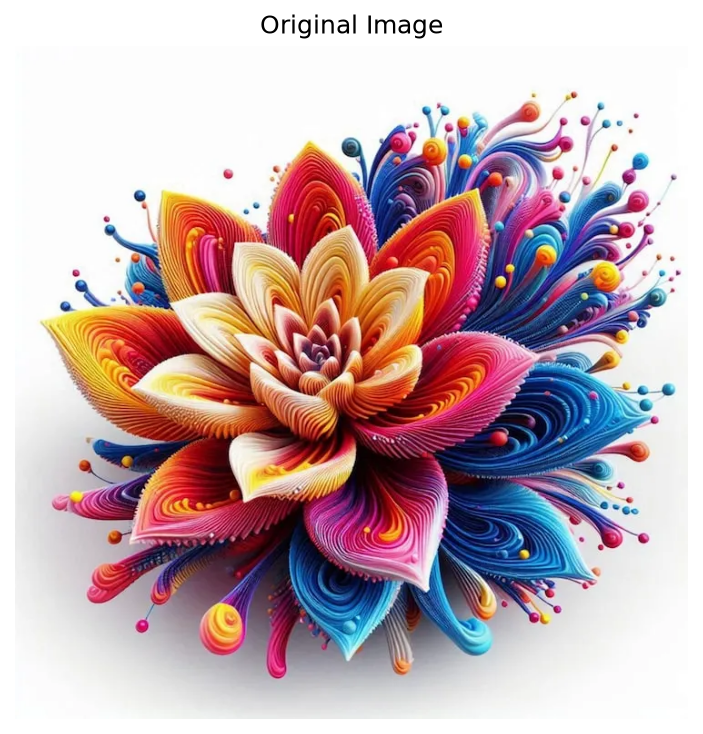
\includegraphics[width=0.55\textwidth]{figures/fig_part2_original.png}
    \caption{Original Image (\texttt{sample.jpg}) rendered in RGB color space.}
    \label{fig:original}
\end{figure}

\textbf{Think Before Moving Ahead}

\textbf{Question:} \textit{Is Python storing this image as a photograph or as numbers?}

\textbf{Answer:} Python stores the image strictly as a discrete multi-dimensional numerical array (\texttt{numpy.ndarray}) containing numerical pixel intensities (0 to 255) across grid coordinates $(y, x)$ and color channels. It does not store an analog photograph.

% ============================================================
% Part 3
% ============================================================
\subsection*{Part 3 — Explore Image Properties}

\begin{lstlisting}[style=code]
print('Data type:', type(img))
print('Shape:', img.shape)
print('Data type of pixels:', img.dtype)
print('Minimum pixel value:', img.min())
print('Maximum pixel value:', img.max())
\end{lstlisting}

\begin{lstlisting}[style=output]
Data type: <class 'numpy.ndarray'>
Shape: (740, 740, 3)
Data type of pixels: uint8
Minimum pixel value: 0
Maximum pixel value: 255
\end{lstlisting}

\textbf{Understand the Output}

For a color image with shape $(height, width, 3)$:
\begin{itemize}
    \setlength\itemsep{0pt}
    \item Height = number of rows ($740$)
    \item Width = number of columns ($740$)
    \item 3 = color channels (Blue, Green, Red in OpenCV)
    \item \texttt{uint8} means each channel intensity is stored using an 8-bit unsigned integer.
\end{itemize}

For an 8-bit image, $L = 2^8 = 256$, so the standard intensity range is $[0, 255]$.

\textbf{Think:} \textit{Why can't a \texttt{uint8} image store the value 300?}

\textbf{Answer:} A \texttt{uint8} data type allocates 8 binary bits per memory cell. The maximum value that can be represented with 8 unsigned bits is $2^8 - 1 = 255$. Any numerical value exceeding 255 overflows the bit register, wrapping around modulo 256 ($300 \pmod{256} = 44$).

% ============================================================
% Part 4
% ============================================================
\subsection*{Part 4 — Convert the Image to Grayscale}

\begin{lstlisting}[style=code]
gray = cv2.cvtColor(img, cv2.COLOR_BGR2GRAY)

plt.figure(figsize=(10, 4))

plt.subplot(1, 2, 1)
plt.imshow(cv2.cvtColor(img, cv2.COLOR_BGR2RGB))
plt.title('Color Image')
plt.axis('off')

plt.subplot(1, 2, 2)
plt.imshow(gray, cmap='gray')
plt.title('Grayscale Image')
plt.axis('off')

plt.tight_layout()
plt.show()

print('Color shape:', img.shape)
print('Grayscale shape:', gray.shape)
\end{lstlisting}

\begin{lstlisting}[style=output]
Color shape: (740, 740, 3)
Grayscale shape: (740, 740)
\end{lstlisting}

\begin{figure}[H]
    \centering
    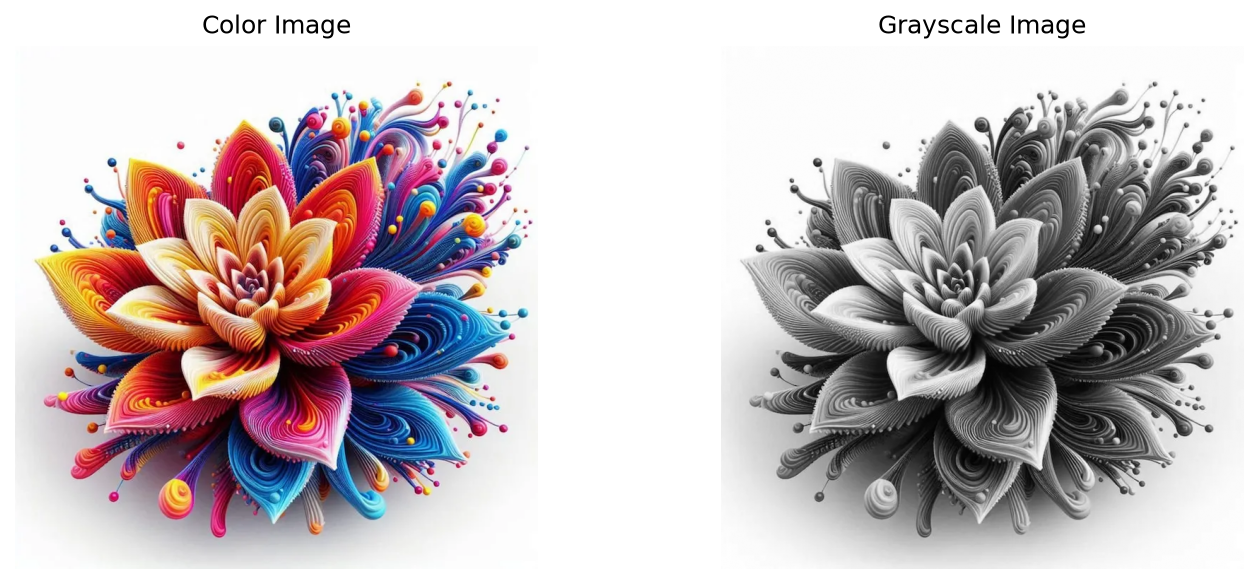
\includegraphics[width=0.85\textwidth]{figures/fig_part4_grayscale.png}
    \caption{Side-by-side visualization of Color Image vs. Grayscale Image.}
    \label{fig:grayscale}
\end{figure}

\textbf{Think:} \textit{Why did the third dimension disappear after converting to grayscale?}

\textbf{Answer:} The third dimension in the color array corresponds to the three distinct spectral color channels (B, G, R). Converting to grayscale combines these color channels into a single scalar luminance value per pixel using the standard perceptual weighting equation:
\begin{equation}
Y = 0.299R + 0.587G + 0.114B
\end{equation}
Consequently, each spatial coordinate $(y, x)$ requires only a single scalar intensity, reducing the array shape from $(H, W, 3)$ to a 2D matrix $(H, W)$.

% ============================================================
% Part 5
% ============================================================
\subsection*{Part 5 — See the Image as a Matrix}
A digital grayscale image is a matrix of intensity values.

\begin{lstlisting}[style=code]
# Grayscale image as a 2D matrix of pixel intensity values
print('Grayscale image slice (top-left 5x5 matrix):\n', gray[:5, :5])
\end{lstlisting}

\begin{lstlisting}[style=output]
Grayscale image slice (top-left 5x5 matrix):
 [[254 254 254 254 254]
 [254 254 254 254 254]
 [254 254 254 254 254]
 [254 254 254 254 254]
 [254 254 254 254 254]]
\end{lstlisting}

\textbf{Pixel Access}\\
Remember: NumPy uses $[row, column]$, i.e., $[y, x]$.

\begin{lstlisting}[style=code]
# Access pixel intensity at row y=100, column x=100
y, x = 100, 100
print(f'Pixel value at (row={y}, col={x}): {gray[y, x]}')
\end{lstlisting}

\begin{lstlisting}[style=output]
Pixel value at (row=100, col=100): 253
\end{lstlisting}

% ============================================================
% Part 6
% ============================================================
\subsection*{Part 6 — Modify One Pixel}
The following experiment changes only one pixel to white.

\begin{lstlisting}[style=code]
modified_img = gray.copy()
modified_img[100, 100] = 255

print('Original pixel value at (100, 100):', gray[100, 100])
print('Modified pixel value at (100, 100):', modified_img[100, 100])

plt.figure(figsize=(5, 4))
plt.imshow(modified_img, cmap='gray')
plt.title('Modified Image (One pixel changed to white)')
plt.axis('off')
plt.show()
\end{lstlisting}

\begin{lstlisting}[style=output]
Original pixel value at (100, 100): 253
Modified pixel value at (100, 100): 255
\end{lstlisting}

\begin{figure}[H]
    \centering
    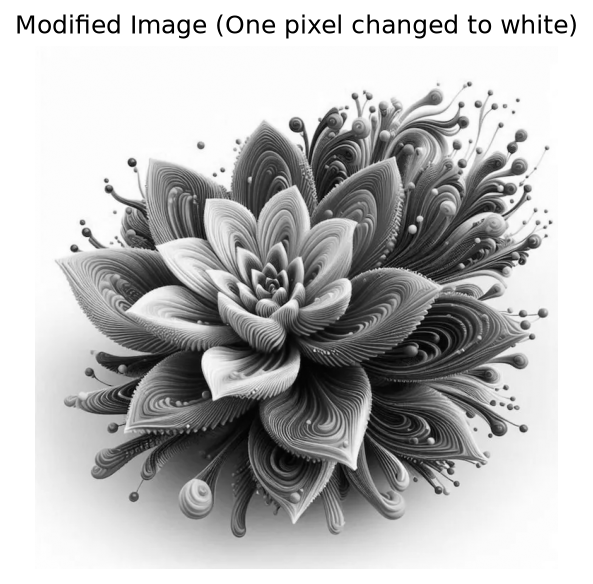
\includegraphics[width=0.45\textwidth]{figures/fig_part6_modified.png}
    \caption{Modified Grayscale Image with pixel $(100, 100)$ set to 255.}
    \label{fig:modified}
\end{figure}

\textbf{Think:} \textit{Only one number changed. Why is the change difficult to notice in the complete image?}

\textbf{Answer:} The image consists of $740 \times 740 = 547,600$ total pixels. A modification to a single pixel occupies less than $0.00018\%$ of the spatial area. Furthermore, the human visual system perceives macro features, textures, and contrast gradients over neighborhoods rather than isolated single-pixel discrepancies.

% ============================================================
% Part 7
% ============================================================
\subsection*{Part 7 — Intensity Transformation: Negative}
For an 8-bit grayscale image:
\begin{equation}
s = 255 - r
\end{equation}
where $r$ is the input intensity and $s$ is the output intensity.

\begin{lstlisting}[style=code]
negative_img = 255 - gray

plt.figure(figsize=(10, 4))
plt.subplot(1, 2, 1)
plt.imshow(gray, cmap='gray')
plt.title('Grayscale Image')
plt.axis('off')

plt.subplot(1, 2, 2)
plt.imshow(negative_img, cmap='gray')
plt.title('Negative Image')
plt.axis('off')

plt.tight_layout()
plt.show()
\end{lstlisting}

\begin{figure}[H]
    \centering
    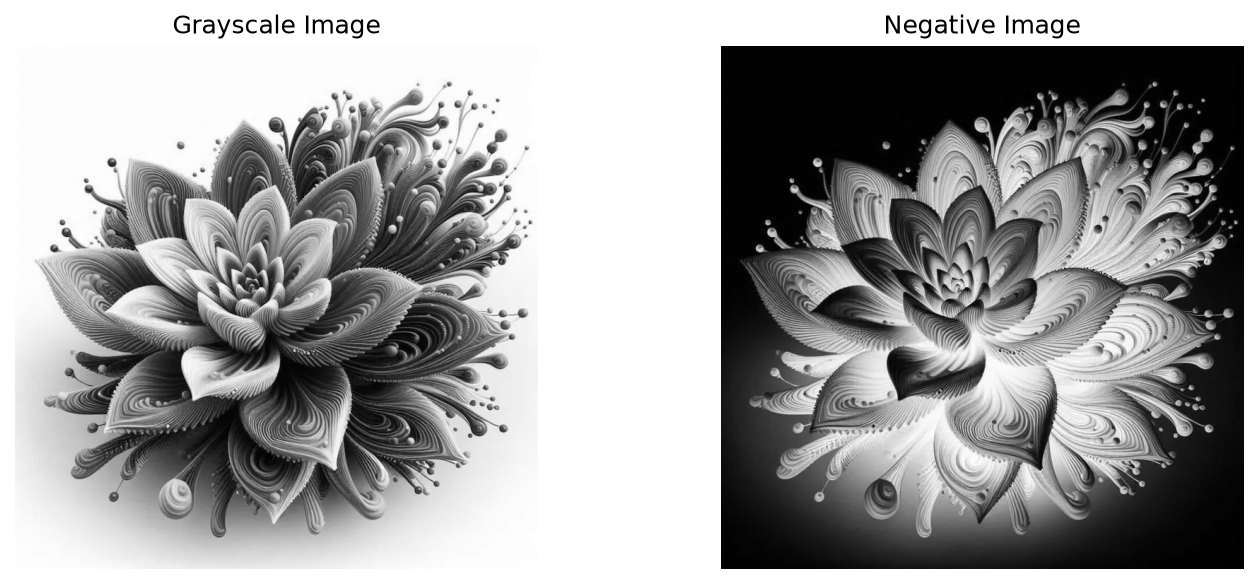
\includegraphics[width=0.85\textwidth]{figures/fig_part7_negative.png}
    \caption{Original Grayscale Image compared with its Photographic Negative ($s = 255 - r$).}
    \label{fig:negative}
\end{figure}

\textbf{Think:} \textit{Why does black become white and white become black?}

\textbf{Answer:} In an 8-bit scale, pure black has intensity $r = 0$, resulting in $s = 255 - 0 = 255$ (pure white). Pure white has intensity $r = 255$, resulting in $s = 255 - 255 = 0$ (pure black). The linear transformation reflects all intensity levels across the dynamic range midpoint ($127.5$).

% ============================================================
% Part 8
% ============================================================
\subsection*{Part 8 — Brightness Transformation}
Increase brightness by 50:
\begin{equation}
s = r + 50
\end{equation}
Because an 8-bit image cannot contain values above 255, clipping is required.

\begin{lstlisting}[style=code]
bright_img = np.clip(gray.astype(np.int16) + 50, 0, 255).astype(np.uint8)

plt.figure(figsize=(10, 4))
plt.subplot(1, 2, 1)
plt.imshow(gray, cmap='gray')
plt.title('Original Grayscale')
plt.axis('off')

plt.subplot(1, 2, 2)
plt.imshow(bright_img, cmap='gray')
plt.title('Brightened Image (+50)')
plt.axis('off')

plt.tight_layout()
plt.show()
\end{lstlisting}

\begin{figure}[H]
    \centering
    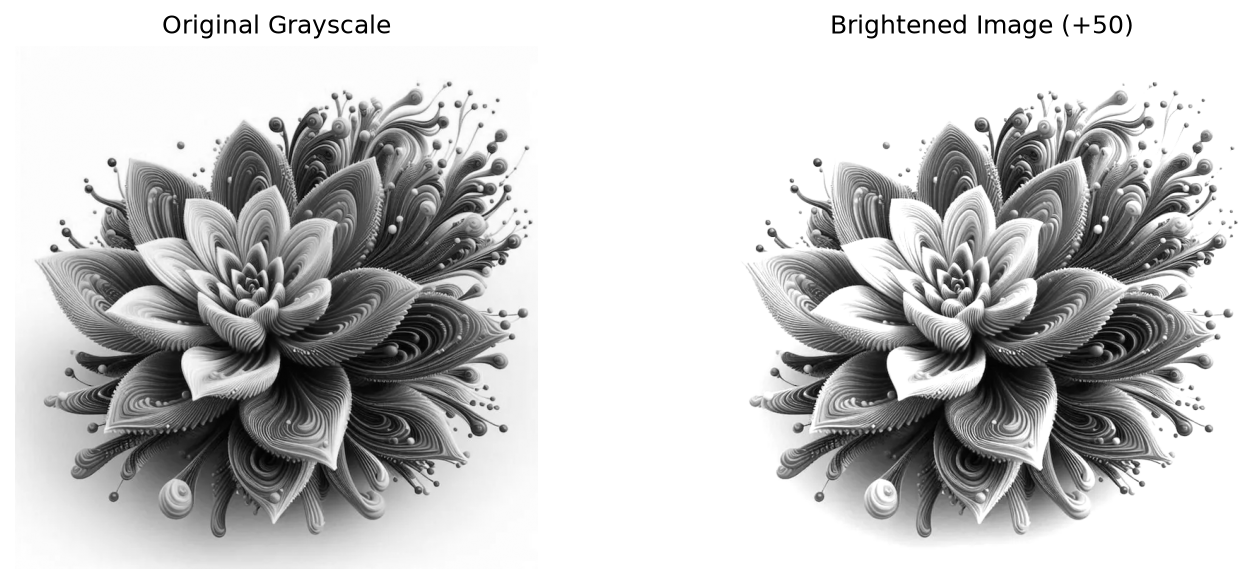
\includegraphics[width=0.85\textwidth]{figures/fig_part8_brightened.png}
    \caption{Original Grayscale vs. Brightened Image ($+50$ intensity with clipping).}
    \label{fig:brightened}
\end{figure}

\textbf{Think:} \textit{Why is \texttt{np.clip()} necessary here?}

\textbf{Answer:} If an intensity value already exceeds 205, adding 50 produces a sum greater than 255. In native \texttt{uint8} arithmetic without clipping, numbers wrap around modulo 256 ($210 + 50 = 260 \equiv 4$), turning bright highlights into dark spots. Casting to a larger signed integer and applying \texttt{np.clip(..., 0, 255)} ensures values saturate at 255 rather than overflowing.

% ============================================================
% Part 9
% ============================================================
\subsection*{Part 9 — Thresholding}
A simple threshold transforms a grayscale image into a binary image:
\begin{equation}
s(x,y) = \begin{cases} 255, & r(x,y) > T \\ 0, & r(x,y) \le T \end{cases}
\end{equation}

\begin{lstlisting}[style=code]
thresholds = [50, 100, 180, 220]

plt.figure(figsize=(14, 4))
for idx, T in enumerate(thresholds, 1):
    binary_img = np.where(gray > T, 255, 0).astype(np.uint8)
    plt.subplot(1, 4, idx)
    plt.imshow(binary_img, cmap='gray')
    plt.title(f'Threshold T = {T}')
    plt.axis('off')

plt.tight_layout()
plt.show()
\end{lstlisting}

\begin{figure}[H]
    \centering
    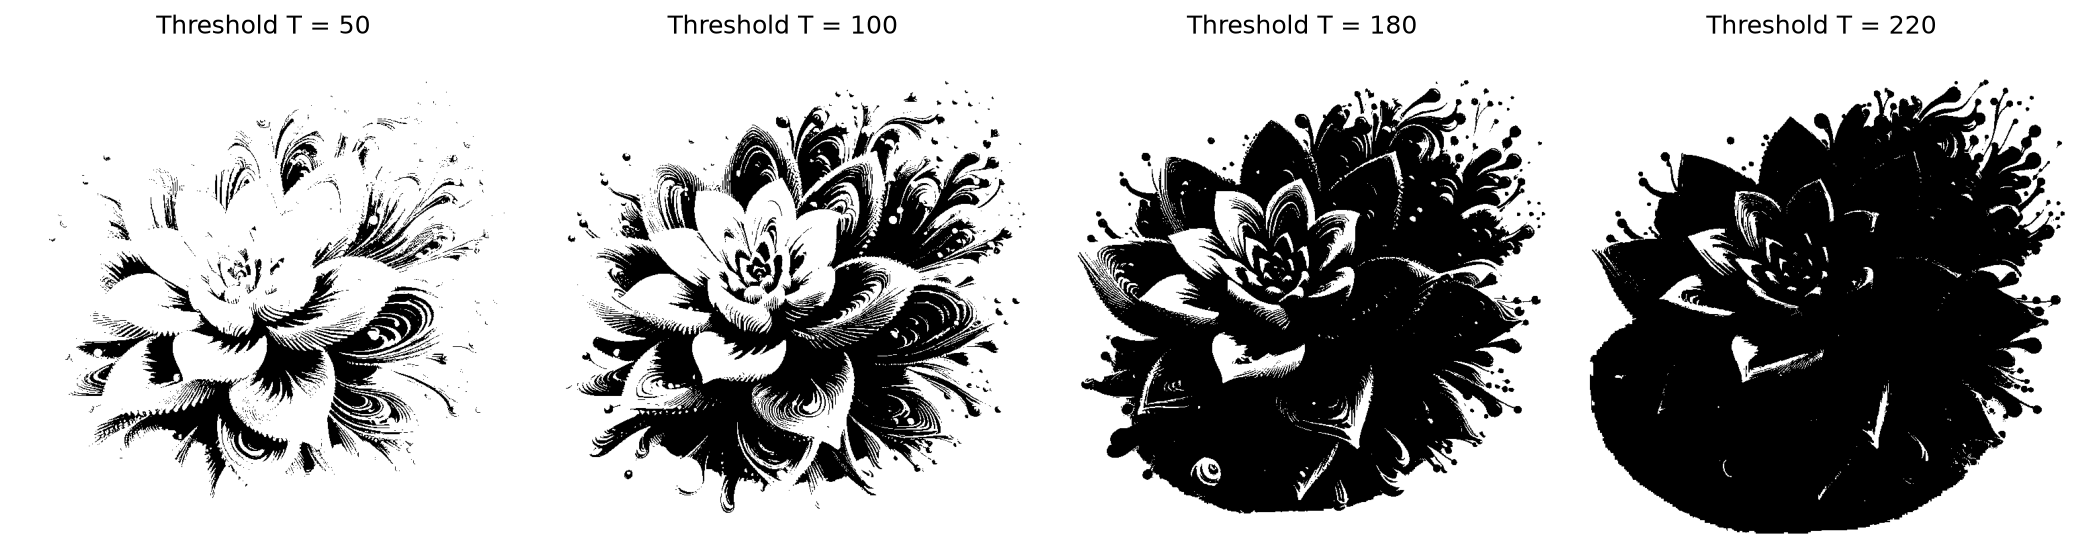
\includegraphics[width=0.95\textwidth]{figures/fig_part9_thresholds.png}
    \caption{Binary Thresholding Results across varying thresholds $T \in \{50, 100, 180, 220\}$.}
    \label{fig:thresholds}
\end{figure}

\textbf{Investigation \& Think:} \textit{Change $T$ to 50, 100, 180, and 220. Why does changing the threshold change the visible object/region?}

\textbf{Answer:} The threshold parameter $T$ determines the decision boundary for binary classification between foreground and background. At low thresholds ($T = 50$), pixels with even mild brightness become white, capturing broad regions. As $T$ increases ($180, 220$), only the brightest specular highlights exceed $T$, causing darker and mid-tone regions to turn black.

% ============================================================
% Part 10
% ============================================================
\subsection*{Part 10 — Histogram}

\begin{lstlisting}[style=code]
plt.figure(figsize=(7, 4))
plt.hist(gray.ravel(), bins=256, range=[0, 256], color='gray')
plt.title('Grayscale Intensity Histogram')
plt.xlabel('Intensity Value')
plt.ylabel('Pixel Count')
plt.grid(axis='y', alpha=0.5)
plt.show()
\end{lstlisting}

\begin{figure}[H]
    \centering
    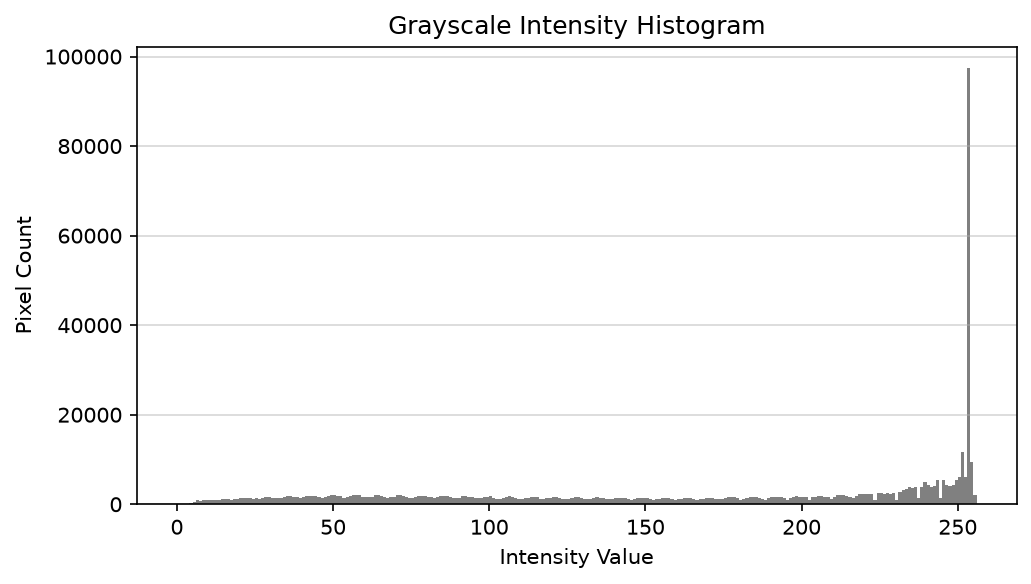
\includegraphics[width=0.60\textwidth]{figures/fig_part10_histogram.png}
    \caption{Grayscale Pixel Intensity Distribution Histogram.}
    \label{fig:histogram}
\end{figure}

\textbf{Think:} \textit{Without looking at the image, what information can the histogram tell you about the distribution of pixel intensities?}

\textbf{Answer:} The histogram reveals the dynamic range and global illumination characteristics of the scene:
\begin{itemize}
    \setlength\itemsep{0pt}
    \item \textbf{Brightness / Exposure:} Peaks skewed towards 0 signify an underexposed (dark) image, whereas peaks concentrated near 255 indicate overexposure.
    \item \textbf{Contrast:} A narrow cluster indicates low contrast, while a spread distribution across the full $[0, 255]$ range denotes high dynamic contrast.
    \item \textbf{Modality:} Multiple distinct peaks imply distinct foreground/background regions suitable for segmentation.
\end{itemize}

% ============================================================
% Part 11
% ============================================================
\subsection*{Part 11 — Cropping and Resizing}

\begin{lstlisting}[style=code]
h, w = gray.shape

# Crop central region
cropped_img = gray[h//4:3*h//4, w//4:3*w//4]

# Resize to half width and height
resized_img = cv2.resize(gray, (w // 2, h // 2))

plt.figure(figsize=(12, 4))
plt.subplot(1, 3, 1)
plt.imshow(gray, cmap='gray')
plt.title(f'Original Grayscale ({w}x{h})')
plt.axis('off')

plt.subplot(1, 3, 2)
plt.imshow(cropped_img, cmap='gray')
plt.title(f'Cropped Image ({cropped_img.shape[1]}x{cropped_img.shape[0]})')
plt.axis('off')

plt.subplot(1, 3, 3)
plt.imshow(resized_img, cmap='gray')
plt.title(f'Resized Image ({resized_img.shape[1]}x{resized_img.shape[0]})')
plt.axis('off')

plt.tight_layout()
plt.show()
\end{lstlisting}

\begin{figure}[H]
    \centering
    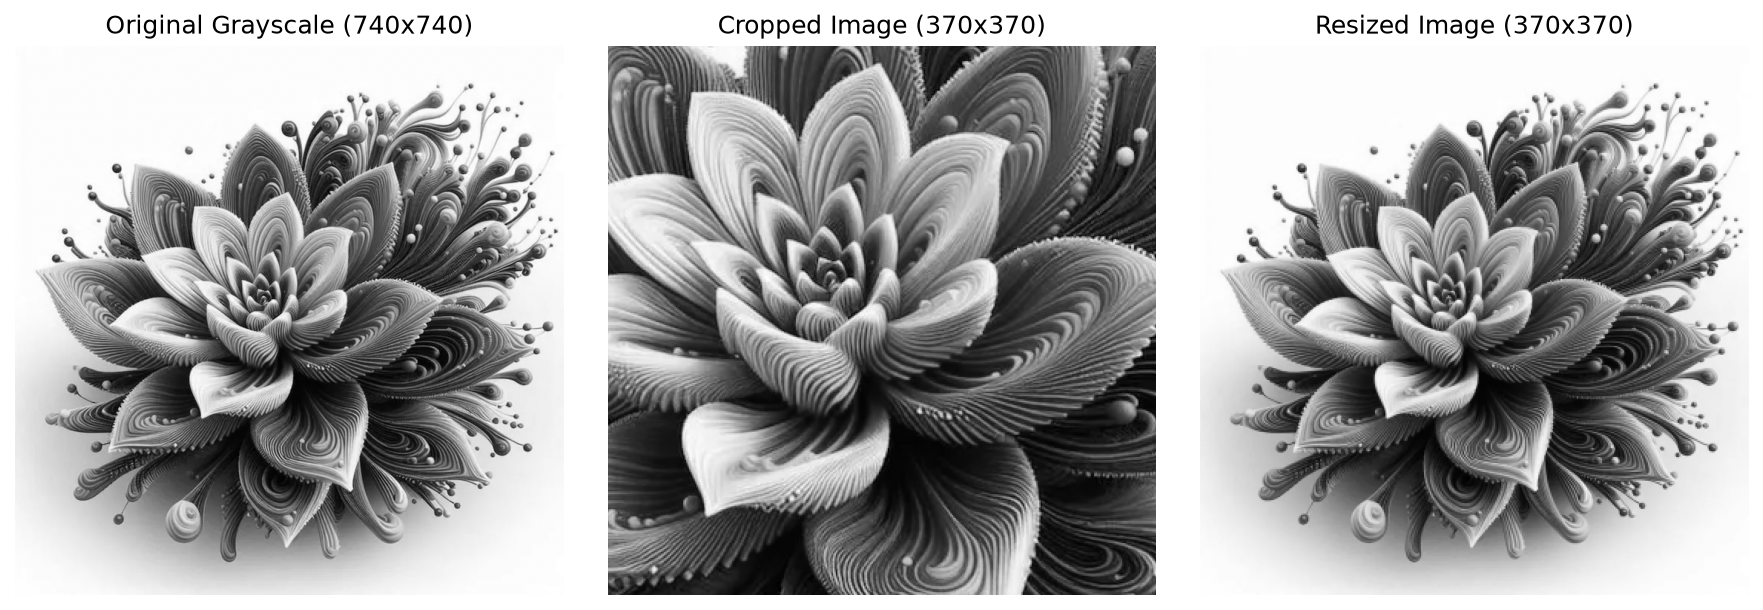
\includegraphics[width=0.92\textwidth]{figures/fig_part11_crop_resize.png}
    \caption{Comparison of Original Image ($740\times740$), Center Cropped Sub-matrix ($370\times370$), and Resized Image ($370\times370$).}
    \label{fig:crop_resize}
\end{figure}

\textbf{Think:} \textit{Which operation changes the spatial dimensions? Does resizing necessarily create new image information?}

\textbf{Answer:} Both operations alter spatial dimensions: cropping extracts a smaller sub-matrix, reducing resolution and field of view, while resizing resamples the entire field of view onto a different grid resolution. Resizing does \textit{not} generate new optical information; downsampling attenuates high-frequency detail, while upsampling merely interpolates existing pixel values.

% ============================================================
% Part 12
% ============================================================
\subsection*{Part 12 — Add Salt-and-Pepper Noise}
The following creates impulse noise by randomly changing some pixels to 0 or 255.

\begin{lstlisting}[style=code]
np.random.seed(42)
noisy_img = gray.copy()
prob = 0.05  # 5% impulse noise

rnd = np.random.rand(*gray.shape)
noisy_img[rnd < (prob / 2)] = 0                      # Pepper (0)
noisy_img[(rnd >= (prob / 2)) & (rnd < prob)] = 255   # Salt (255)

plt.figure(figsize=(6, 5))
plt.imshow(noisy_img, cmap='gray')
plt.title('Salt-and-Pepper Noisy Image')
plt.axis('off')
plt.show()
\end{lstlisting}

\begin{figure}[H]
    \centering
    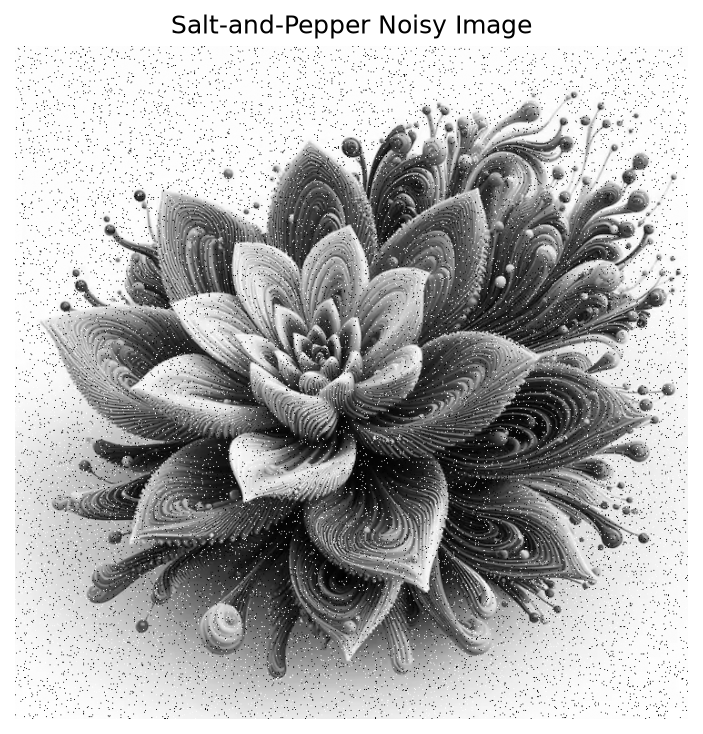
\includegraphics[width=0.50\textwidth]{figures/fig_part12_noisy.png}
    \caption{Image corrupted with 5\% Salt-and-Pepper Impulse Noise.}
    \label{fig:noise}
\end{figure}

% ============================================================
% Part 13
% ============================================================
\subsection*{Part 13 — Mean vs Median Filtering}
Now connect the experiment to order-statistic filtering.

\begin{lstlisting}[style=code]
# Mean filter using 3x3 window
mean_filtered = cv2.blur(noisy_img, (3, 3))

# Median filter using 3x3 window
median_filtered = cv2.medianBlur(noisy_img, 3)

plt.figure(figsize=(14, 5))
plt.subplot(1, 3, 1)
plt.imshow(noisy_img, cmap='gray')
plt.title('Noisy Image')
plt.axis('off')

plt.subplot(1, 3, 2)
plt.imshow(mean_filtered, cmap='gray')
plt.title('Mean Filtered (3x3)')
plt.axis('off')

plt.subplot(1, 3, 3)
plt.imshow(median_filtered, cmap='gray')
plt.title('Median Filtered (3x3)')
plt.axis('off')

plt.tight_layout()
plt.show()
\end{lstlisting}

\begin{figure}[H]
    \centering
    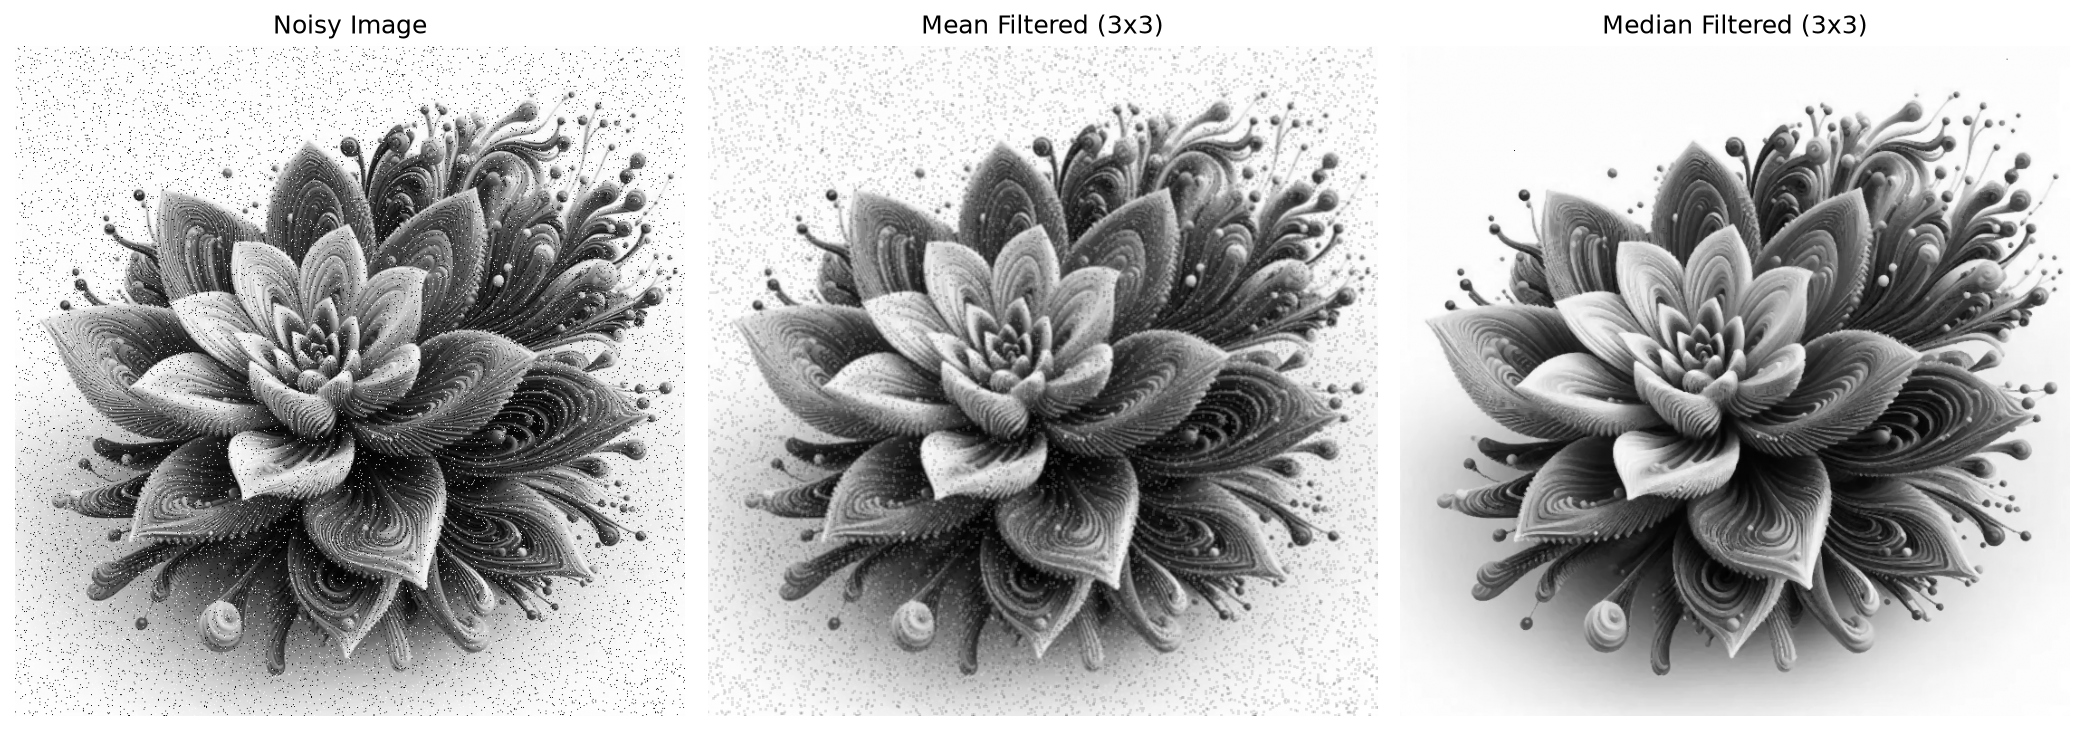
\includegraphics[width=0.95\textwidth]{figures/fig_part13_filtering.png}
    \caption{Comparison of Impulse Noisy Image, Linear Mean Filtered Image ($3\times3$), and Order-Statistic Median Filtered Image ($3\times3$).}
    \label{fig:filtering}
\end{figure}

\textbf{Critical Thinking}

Compare the noisy image, mean-filtered image and median-filtered image:
\begin{enumerate}
    \item \textbf{Which filter removes the salt-and-pepper noise more effectively?}\\
    \textit{Answer:} The \textbf{median filter} removes salt-and-pepper noise far more effectively. Because impulse noise consists of extreme outliers (0 and 255), sorting the neighborhood ranks these outliers at the extremes, leaving a representative median value that restores the true underlying intensity.
    
    \item \textbf{Which filter preserves edges better?}\\
    \textit{Answer:} The \textbf{median filter} preserves sharp edges significantly better. Linear mean filtering averages across edge boundaries, creating blur and halo artifacts, whereas the median filter maintains step discontinuities.
    
    \item \textbf{Why can an extreme value such as 255 strongly affect the mean but have much less effect on the median?}\\
    \textit{Answer:} The mean is a linear sum $\frac{1}{N}\sum x_i$. An extreme outlier ($255$) pulls the arithmetic mean heavily towards the outlier. In contrast, the median is an order-statistic rank metric that depends solely on the middle value of the sorted sequence, completely ignoring the magnitude of tail outliers.
    
    \item \textbf{What do you expect if the window is changed from $3\times3$ to $7\times7$?}\\
    \textit{Answer:} A $7\times7$ window increases the neighborhood size from 9 to 49 pixels. For the mean filter, this causes severe image blurring and loss of high-frequency detail. For the median filter, a $7\times7$ window can suppress higher noise densities but causes rounding of fine corners and erosion of thin lines.
\end{enumerate}

% ============================================================
% Part 14
% ============================================================
\subsection*{Part 14 — Manual Order-Statistic Exercise}
Consider the following $3\times3$ neighborhood:
\begin{equation}
\mathbf{N} = \begin{bmatrix} 42 & 43 & 44 \\ 43 & 255 & 45 \\ 44 & 45 & 46 \end{bmatrix}
\end{equation}

\textbf{Step 1: Sorted Neighborhood Sequence}\\
Arranging the 9 intensity values in ascending order:
\begin{equation}
\{ 42,\, 43,\, 43,\, 44,\, \mathbf{44},\, 45,\, 45,\, 46,\, 255 \}
\end{equation}

\textbf{Step 2: Manual Mathematical Calculations}
\begin{itemize}
    \setlength\itemsep{0pt}
    \item \textbf{Minimum:} $\min = 42$
    \item \textbf{Maximum:} $\max = 255$
    \item \textbf{Median:} The 5th element in the 9-element sorted list is $44$.
    \item \textbf{Mean:}
    \begin{equation}
    \mu = \frac{42 + 43 + 44 + 43 + 255 + 45 + 44 + 45 + 46}{9} = \frac{607}{9} \approx 67.44
    \end{equation}
    \item \textbf{Midpoint:}
    \begin{equation}
    \text{Midpoint} = \frac{\min + \max}{2} = \frac{42 + 255}{2} = \frac{297}{2} = 148.5
    \end{equation}
\end{itemize}

\begin{table}[H]
\centering
\begin{tabular}{|l|c|c|}
\hline
\textbf{Statistic Metric} & \textbf{Theoretical Formula} & \textbf{Calculated Value} \\ \hline
Minimum & $\min(\mathbf{N})$ & 42 \\ \hline
Maximum & $\max(\mathbf{N})$ & 255 \\ \hline
Median & $\text{median}(\mathbf{N})$ & 44 \\ \hline
Mean & $\frac{1}{9}\sum_{i=1}^9 x_i$ & 67.44 \\ \hline
Midpoint & $\frac{\min + \max}{2}$ & 148.5 \\ \hline
\end{tabular}
\caption{Summary of Order-Statistic Values for the $3\times3$ Neighborhood Matrix.}
\label{tab:order_stats}
\end{table}

\textbf{Step 3: Python Execution Verification}
\begin{lstlisting}[style=code]
neighborhood = np.array([
    [42, 43, 44],
    [43, 255, 45],
    [44, 45, 46]
])

print('Neighborhood Matrix:\n', neighborhood)
print('---')
print('Minimum: ', np.min(neighborhood))
print('Maximum: ', np.max(neighborhood))
print('Median:  ', np.median(neighborhood))
print('Mean:    ', round(float(np.mean(neighborhood)), 2))
print('Midpoint:', (int(np.max(neighborhood)) + int(np.min(neighborhood))) / 2.0)
\end{lstlisting}

\begin{lstlisting}[style=output]
Neighborhood Matrix:
 [[ 42  43  44]
 [ 43 255  45]
 [ 44  45  46]]
---
Minimum:  42
Maximum:  255
Median:   44.0
Mean:     67.44
Midpoint: 148.5
\end{lstlisting}

\vfill
\hrule
\begin{center}
    \small \textit{End of Lab Report — Computer Vision and Image Processing (CSDS119)}
\end{center}

\end{document}
